\documentclass[a4paper]{article}
\usepackage[pdftex]{graphicx}
\usepackage[utf8]{inputenc}
\usepackage{enumerate}
\usepackage{icomma}
\usepackage{amssymb}
\usepackage{tikz}
\usepackage{href-ul}
\hypersetup{
	colorlinks=true,
	linkcolor=blue,
	urlcolor=blue}
\usepackage{geometry}
\geometry{a4paper, top=15mm, left=15mm, right=15mm, bottom=15mm,
	headsep=10mm, footskip=12mm}

\begin{document}
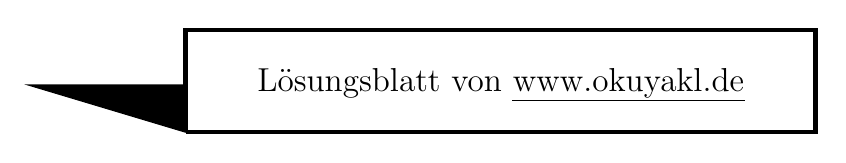
\begin{tikzpicture}(10,3)
	\draw[ultra thick](2,0) --(10,0) -- (10,1.3) --(2,1.3) -- (2,0);
	\draw[fill=black](2,0)-- (0,.6) -- (2,.6) -- (2,0);
	\node at (6,.6) {\large Lösungsblatt von \href{https://www.okuyakl.de}{www.okuyakl.de}};
\end{tikzpicture}
\vspace{0.5 cm}

\noindent{\bf Aufgabe 1.}\\
Diese Abbildung beschreibt eine Drehung um den Ursprung um $\sin^{-1}0,80 = 53,1^\circ$.

\noindent{\bf Aufgabe 2.}\\
Wir vergleichen mit der Spiegelmatrix aus der Formelsammlung:
$$-0,71 = \cos 2\alpha \quad \Rightarrow \quad \alpha = {1 \over 2} \cdot \cos^{-1} (-0,71) =67,6^\circ$$
Dann folgt:
$$z=0,71 \quad y= -0,71$$
Die Spiegelachse hat die Steigung:
$$m= \tan \alpha = \tan 67,6^\circ = 2,4 $$
Damit ist die Spiegelachse:
$$g:\quad y=2,4x$$

\noindent{\bf Aufgabe 3.}\\
Der Steigungswinkel der Geraden ist:
$$\alpha = \tan^{-1}\left(-{2 \over 3 }\right) =-33,7^\circ$$
Wir wenden die Spiegelmatrix auf die Gerade h an:
 $$ \left(
\begin{array}{c}
	x'\\
	y'
\end{array}
\right) = 
\left(
\begin{array}{cc}
	\cos 2 \alpha & \sin 2 \alpha \\
    \sin 2 \alpha & -\cos 2 \alpha
\end{array}
\right)
\odot 
\left(
\begin{array}{c}
	x\\
	y
\end{array}
\right)$$

 $$ \left(
 \begin{array}{c}
 x'\\
 y'
 \end{array}
 \right) = 
 \left(
 \begin{array}{cc}
 0,385 & -0,923 \\
 -0,923  & -0,385
 \end{array}
 \right)
 \odot 
 \left(
 \begin{array}{c}
 x\\
 2x +2
 \end{array}
 \right)$$
 
  $$ \left(
  \begin{array}{c}
  x'\\
  y'
  \end{array}
  \right) = 
  \left(
  \begin{array}{cc}
   0,385x -1,846x -1,846\\
  -0,923x - 0,770x-0,770 \\
  
  \end{array}
   \right) = 
   \left(
   \begin{array}{cc}
   -1,461x -1,846\\
   -1,693x -0,77 \\
   \end{array}
  \right)$$
  
  $$
  \renewcommand{\arraystretch}{2}
  \begin{array}{rcll}
  x &=& - 0,684 x' - 1,264 \\
  y' &=& 1,16 x + 2,14 -0,77 &= 1,16x +1,37
  \end{array}
  $$
  Damit ist $$h': y=1,16x+1,37$$
  
 
  \noindent
  \begin{minipage}{0.5\textwidth}
  	 \noindent{\bf Aufgabe 4. a)}\\
  		\includegraphics[width=7 cm]{pasch028}
  \end{minipage}
  \hfill
  \begin{minipage}{0.5\textwidth}
   \noindent{\bf Aufgabe 4. b)}\\
   Wir setzen (-x) in den Funktionsterm ein und erhalten:
   $$f(-x)= (-x)^2 - 2\cdot (-x) +4 = x^2 +2x+4$$
   
   \noindent{\bf Aufgabe 4. c)}\\
   Wir bilden die Umkehrfunktion:
   $$
   \renewcommand{\arraystretch}{2}
   \begin{array}{rcll}
   x &=& y^2+2x+4 \\
   x &=& (y+1)^2 +3 \\
   x-3 &=& (y+1)^2 \\
   \sqrt{x-3} &=& y+1 \\
   \sqrt{x-3}-1 &=& y 
   \end{array}
   $$
  \end{minipage}
  
\begin{center}
	\includegraphics[width=7 cm]{../../viecher/endcomic.pdf}
	
	Hier geht es zurück zum \href{https://www.okuyakl.de/math/m10rsabbL028/aa028.pdf}{Aufgabenblatt}
\end{center}

\end{document}

